\chapter{Title of third chapter}
	\label{CH_03}


\section{This is an example section title which will span two lines both here and in the table of contents}
Further illustration of how chapters are presented.


\subsection{Title of subsection}
Here is a subsection.  The following figure will show up in the `List of Figures'.

\begin{figure}[h] % h places the image 'here' (as long as LaTeX thinks it will fit here well), 't' for top of page, 'b' for bottom of page, 'H' for I WANT IT HERE!!! (regardless of whether the latex compiler thinks it will fit.)
	\centering
	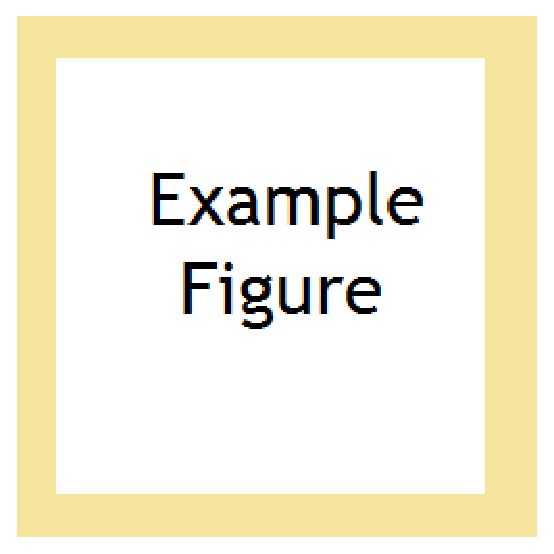
\includegraphics[width=2.0in]{Figures/figure1}
	\caption[Box figure]{A sample image which will show up in the the List of Figures as `Box figure'}
\end{figure}
\begin{table}[t]
	\centering
	\begin{tabular}{|r|l|}
	\hline
	7C0 & hexadecimal \\
	3700 & octal \\ \cline{2-2}
	11111000000 & binary \\
	\hline \hline
	1984 & decimal \\
	\hline
	\end{tabular}
	\caption[Digit representation]{A sample table which will show up in the the List of Tables as `Digit representation table'; it is set to align at the top of a page}
\end{table}

Some paragraph text follows. Some paragraph text follows. Some paragraph text follows. Some paragraph text follows. Some paragraph text follows. Some paragraph text follows. Some paragraph text follows. Some paragraph text follows. Some paragraph text follows. Some paragraph text follows. Some paragraph text follows. Some paragraph text follows. Some paragraph text follows. Some paragraph text follows. Some paragraph text follows. Some paragraph text follows. Some paragraph text follows. Some paragraph text follows. 

\begin{table}[h]
	\centering
	\begin{tabular}{llr}
	\hline
	\multicolumn{2}{c}{Item} \\
	\cline{1-2}
	Animal & Description & Price (\$) \\
	\hline
	Gnat  & per gram & 13.65 \\
	 & each     &  0.01 \\
	Gnu   & stuffed  & 92.50 \\
	Emu   & stuffed  & 33.33 \\
	Armadillo & frozen & 8.99 \\
	\hline
	\end{tabular}
	\caption[Odd foods]{Another table which will show up in the the List of Tables as `Odd foods'; it is set to align ``here" in the text.}
\end{table}



